%% This .tex file was created by Ray Goerke and Henry Ngo for the UBC
%% Physics Society Latex Tutorial Session 2009.  Feel free to use this as
%% a reference or template for your own .tex files.
%%
%% Edited by William Scales for 2013

%---------------------- PREAMBLE ----------------------%

%\documentclass{article}
%\usepackage{amsmath}

% RevTeX4 is the standard APS format
\documentclass[twocolumn,10 pt,showpacs,preprintnumbers,amsmath,amssymb]{revtex4-1}

\usepackage{graphicx} % Allows including figures in ps (or eps) format
\usepackage{dcolumn}  % Align columns on the decimal point
\usepackage{bm}       % Makes math bold

% This is a command definition
\newcommand{\parl}[2]{\frac{\partial #1}{\partial #2}}

%---------------- THE ACTUAL DOCUMENT -----------------%

\begin{document}

\title{Latex Session 2013}

\author{Your name here}
\affiliation{Department of Physics and Astronomy, University of British Columbia \\
             6224 Agricultural Road, Vancouver, British Columbia, Canada, V6T 1Z1}

% If you omit \date{\today}, LaTeX assumes you meant today.  You only
% need this if you want to specify a different date.
\date{\today}

\begin{abstract}
  We demonstrate methods for creating nice-looking PDFs for research
  papers including mathematical formulae, figures, tables, and
  bibliographies using \LaTeX !
\end{abstract}

\maketitle

\section{Introduction}

You can use latex to do all of the things word processors can do, like
\textbf{bold} and \textit{italics}.  We can make fonts that are {\Large
bigger} or even {\Huge bigger} and also fonts that are really {\tiny 
small}.

New paragraphs like this one are automatically indented according to the
document class that you declared at the begining of the file.  Note that
actual indenting in the .tex file is ignored.  You can start or end a
line wherever you want.  \LaTeX~ will only start a new paragraph if you
leave a blank line.  If you want\\ to end\\ a line early\\ you have to
use\\ two backslashes.

This document uses the \texttt{Rev\TeX 4} class, which is the standard for
all APS journals. It is also the standard for PHYS/ASTRO 449, which is
why we are using it here. The options in the square brackets of the
\verb_\documentclass_ command define various properties of the document
including number of columns and global text size. If you want to see
what a simpler format looks like, you can comment out the
\verb_\documentclass_ line in the preamble and uncomment the two lines
above it. You will also have to move the \verb_\maketitle_ command to
just before the abstract, and comment out both lines of the affiliation
command, because of the slightly different way the two document classes
handle titles.

\noindent You can use the \verb_\noindent_ command to force a new
paragraph to not be indented.  Also, notice that above when I wrote
\verb_\noindent_, \LaTeX~ did not interpret it as a command, but as
text.  To do this I used the \verb_\verb_ command.

\section{Equations}

One of the most popular features of \LaTeX~ is the ability to make nice
looking math equations.  Here are some examples: 
\begin{equation}
  \parl{u}{t} = \alpha^2 \parl{^2u}{x^2}
  \label{eqn:heat}
\end{equation}
\begin{equation}
  \int_{\alpha}^{\beta} e^{-\frac{{\Gamma_0}^2\omega b x}{q \sigma \epsilon}}\sin\left(
  \frac{23}{17}\pi x\right)dx
  \label{eqn:random}
\end{equation}
Note that if you give your equations labels, then you can reference them
in the text, like this: Equation~\ref{eqn:heat} and
Equation~\ref{eqn:random}.  The advantage of using these types of
references is that they will always refer to the correct equation, even
if you add more in later or rearrange them.

There are no limits to what you can do with \LaTeX~ equations. You can
make matrices and vectors or whatever you like, just Google it.

\subsection{Inline equations}

Sometimes you want to have a short bit of math inside the text, like
this: $h\nu = \hbar\omega$.  To do this you can surround your math with
\$'s.

\subsection{Align}

If you want to have a derivation that take multiple lines and have all the equal
signs line up, we can use the align environment:
\begin{align*}
  2x^2 + 3(x-1)(x-2) &= 2x^2 + 3(x^2-3x+2)\\
                     &= 2x^2 + 3x^2 - 9x + 6\\
                     &= 5x^2 - 9x + 6
\end{align*}
Note that with both the \verb_eqaution_ and \verb_align_ environments,
if you put an asterix after the name in the begin statments (e.g.
\verb_\begin{align*}_), the equations will not be numbered.  The same
thing works for sections and subsetions. For example the next section
has no number:

\section*{Floats}

Floats are things that \LaTeX~ will intelligently place within your
text.  The most common types of floats are figures and tables.

\subsection{Figures}

The standard package to use for images is graphicx. We start by creating
a \texttt{figure} environment, then a \texttt{center} environment. The
figure environment tells \LaTeX~ ``I am a float, you get to put me
somewhere to make efficient use of space!''. The center environment
ensures it's centred in the column. We use the \verb_\includegraphics_
command to include the actual figure.  If you're using \texttt{LaTeX},
not \texttt{PDFLaTeX} the figure should be in postscript (.ps or .eps)
format.  If you're using \texttt{PDFLaTeX}, the figure can be a .jpg,
.png, or .pdf file.  Note that options in square brackets allow you to
scale or rotate the image.  Lastly we add a caption, and give the figure
a label so we can refer to it in the text (see Figure~\ref{fig:exp}).

\begin{figure}
  \centering
  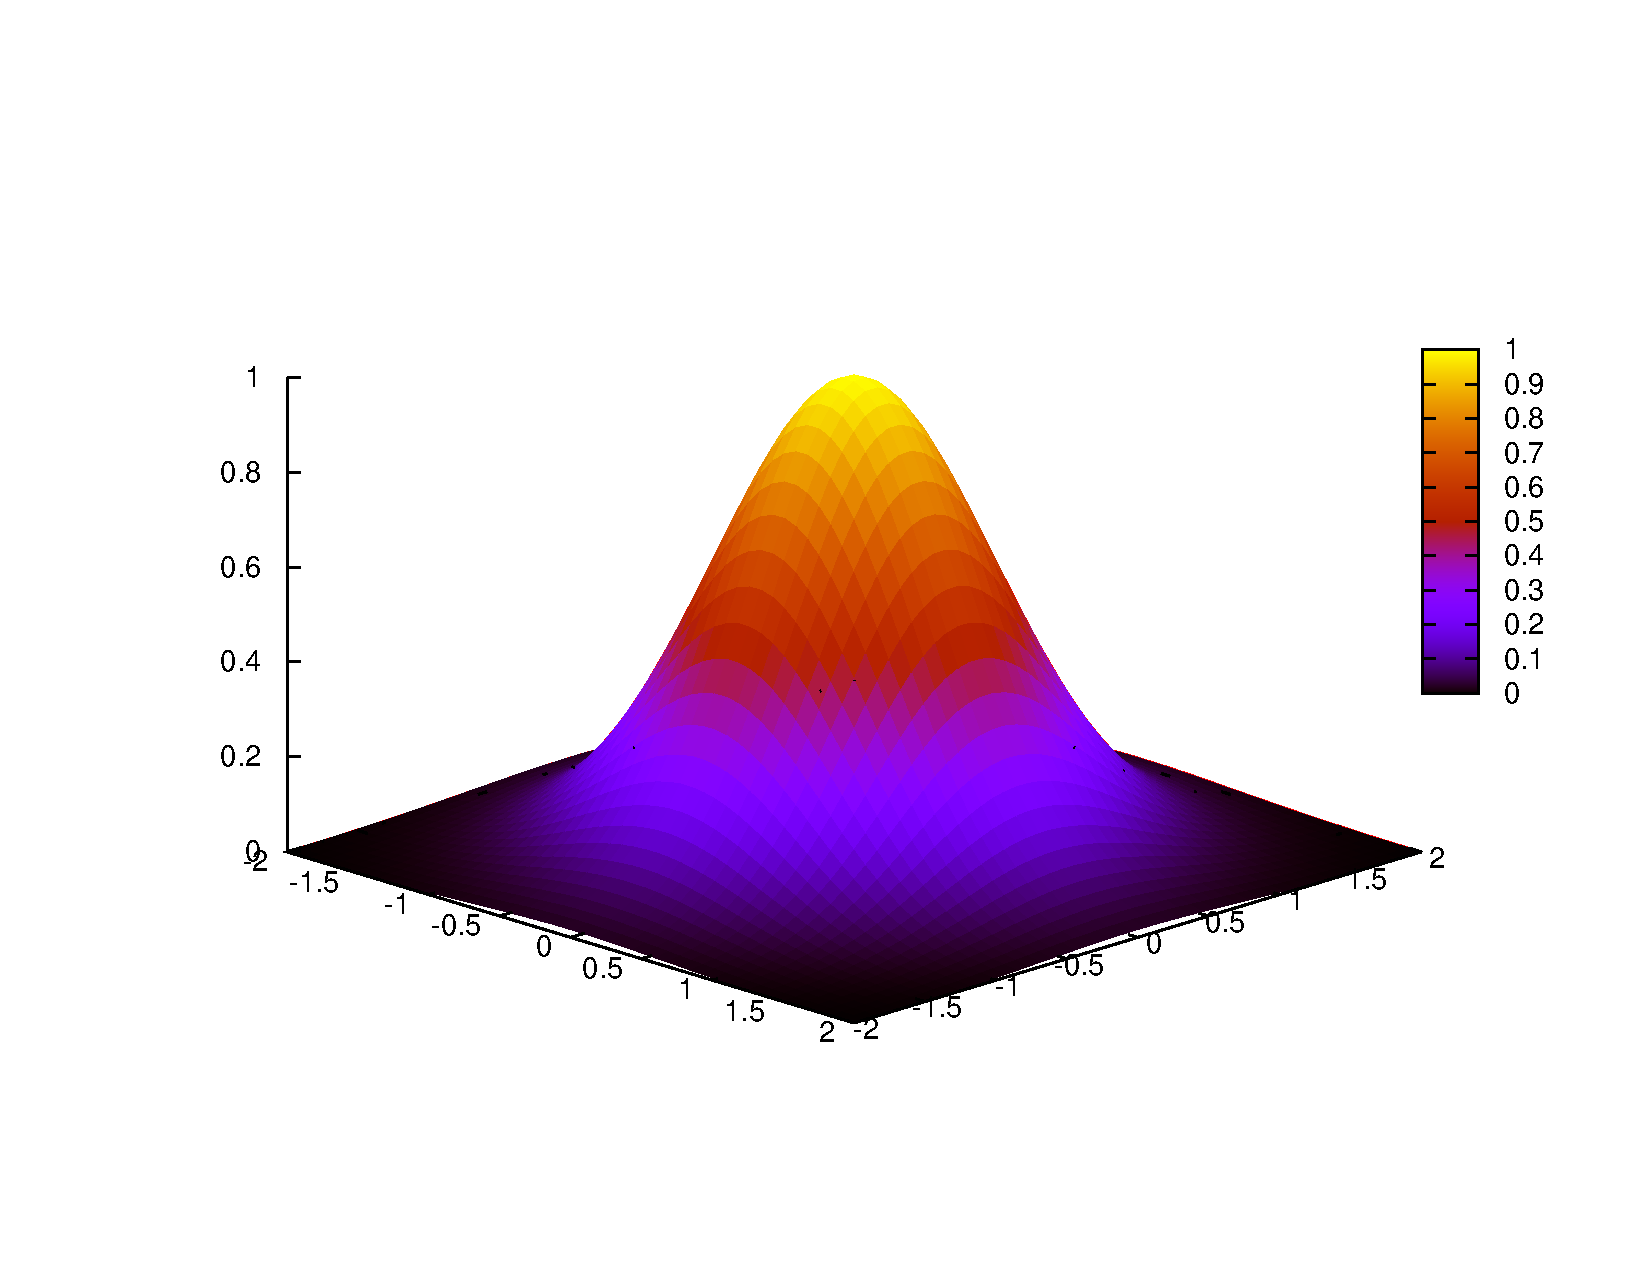
\includegraphics[scale=0.25,angle=-90]{figure.pdf}
  \caption{This is a figure}
  \label{fig:exp}
\end{figure}

\subsection{Tables}

Tables in \LaTeX~ can sometimes seem tedious, but they are very
flexible.  Note that to make a table we need two environments: first we
need the \texttt{table} environment to make a float which can contain,
among other things, captions, and then we need the \texttt{tablular}
environment to actually define the contents of the table.  Technically
you could make a table with just the \texttt{tablular} environment, but
then it would not be placed intelligently like other floats and could
not be referenced like Table~\ref{tbl:sqr}.
\begin{table}
  \centering
  \begin{tabular}{|l|r|} \hline
    $x$  &  $x^2$ \\ \hline
    1    &  1  \\
    2    &  4  \\
    3    &  9  \\
    4    &  16 \\
    5    &  25 \\ \hline
  \end{tabular}
  \caption{This is a table}
  \label{tbl:sqr}
\end{table}
\begin{table}
  \centering
  \begin{tabular}{lr} \hline \hline
    $x$  &  $x^2$\\ \hline
      1    &  1  \\
      2    &  4  \\
      3    &  9  \\
      4    &  16 \\
      5    &  25 \\ \hline
  \end{tabular}
  \caption{This is a trendy table}
  \label{tbl:trendy}
\end{table}
Right after the \verb_\begin{tabular}_ command, we define some options
about the columns.  I have written \texttt{|l|r|}, which means we have
two columns, the first is left-aligned, and the second is right-algined.
The vertical lines or `pipes' for us 'Nix nerds mean that there should
be a vertical line on the outsides of the table and separating the
columns.  In the content of the table, you should write \verb_\hline_
every time you want to a horizontal line, and then separate each column
with an \&.  Also every line that isn't an \verb_\hline_ should be ended
by two backslashses.

Table \ref{tbl:trendy} shows how you can change some of the above
options to make a more trendy looking table.

One last comment on floats is that if you don't like where \LaTeX~ puts
them and you really think it should go HERE, then you can force it to by
putting \texttt{[h]} right after the \verb_\begin{table}_ or
\verb_\begin{figure}_, like Figure~\ref{fig:here}, which should be right
here:
\begin{figure}[h]
    \centering
    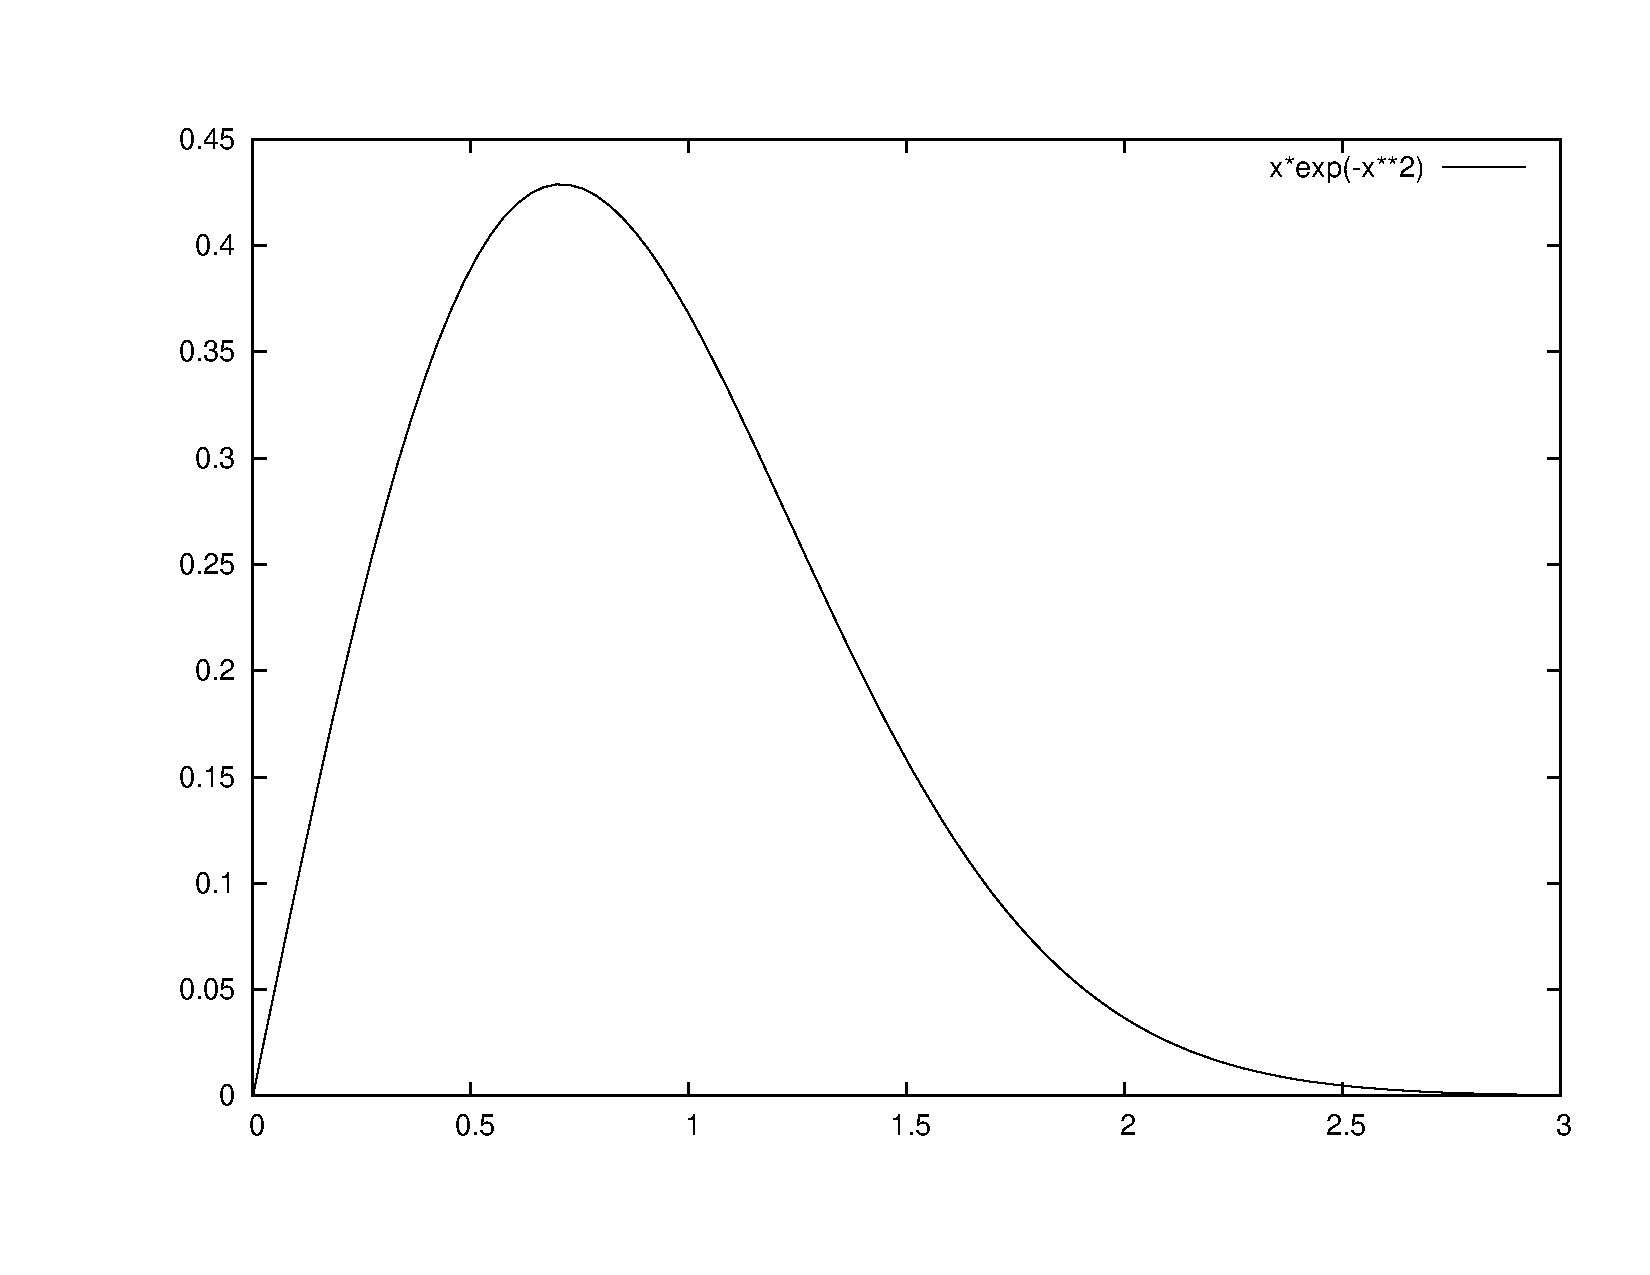
\includegraphics[scale=0.25,angle=-90]{graph.pdf}
    \caption{This is right here}
    \label{fig:here}
\end{figure}

\section{Bibilography}

The best and most flexible way to make a biliography in latex is to use
an extention called Bib\TeX, but that is somewhat complicated and beyond
the scope of this session.  There is a good standard environment which
works well as long as you don't want to get too fancy.  It's called
\texttt{thebibliography} and you can use it to cite things in the
text\cite{smith}.  Note that the number will always be consistent and
will reflect adding or rearranging entries\cite{author}.

\begin{thebibliography}{99}

\bibitem{author} Author, I. N. (Year). Title of the article. Title of the Journal or Periodical, volume number, page numbers.

\bibitem{smith} Smith, L. V. (2000). Referencing articles in APA format. APA Format Weekly, 34, 4-10.

\end{thebibliography}

\end{document}
